\documentclass{article}

\usepackage[french]{babel}
\usepackage[utf8]{inputenc}
\usepackage[T1]{fontenc}
\usepackage{graphicx}
\usepackage{algorithm}
\usepackage{algorithmic}
\usepackage{amsmath}
\usepackage{systeme}
\usepackage{float}
\usepackage{amssymb}
\usepackage{mathrsfs}
\usepackage{color}
\usepackage{fancyhdr}
\usepackage{pdfpages}
\usepackage{layout}
\usepackage{multicol}
\usepackage{setspace}
\usepackage{csvsimple}
\usepackage[table]{xcolor}
\usepackage[colorlinks=true]{hyperref}
\usepackage{tikz, tkz-tab}
\usepackage[top=2cm,bottom=2cm,left=2cm,right=2cm]{geometry}
\usepackage{amsthm}


\usepackage{multicol}

%%%%%%%%%%%%%%%% Lengths %%%%%%%%%%%%%%%%
\setlength{\textwidth}{15.5cm}
\setlength{\evensidemargin}{0.5cm}
\setlength{\oddsidemargin}{0.5cm}

%%%%%%%%%%%%%%%% Variables %%%%%%%%%%%%%%%%
\def\project{4}
\def\title{Non-linear systems of equations and the Newton-Raphson method}
\def\group{3}
\def\team{3}
\def\manager{Lucas Guédon}
\def\secretary{Salim Bekkari}
\def\others{Mohammed Boudali, Imad Boudroua, Simon Bullot}
\singlespace
\begin{document}

%%%%%%%%%%%%%%%% Header %%%%%%%%%%%%%%%%
\noindent\begin{minipage}{0.98\textwidth}
  \vskip 0mm
  \noindent
  { \begin{tabular}{p{6.5cm}}
      {\bfseries \sffamily
        Project \project} \\ 
      {\itshape \title}
    \end{tabular}}
  \hfill 
  \fbox{\begin{tabular}{p{8.4cm}}
      {~\hfill \bfseries \sffamily Group \group\ - Team \team
        \hfill~} \\[2mm] 
      Manager: \manager \\
      Secretary: \secretary \\
      Programmers: \others
    \end{tabular}}
  \vskip 4mm ~

  ~~~\parbox{0.95\textwidth}{\small \textit{Abstract~:} \sffamily The aim of the project is to implement the Newton-Raphson method to solve non-linear systems of equations and apply it to problems.}
  \vskip 1mm ~
\end{minipage}

%%%%%%%%%%%%%%%% Main part %%%%%%%%%%%%%%%%

\section{Newton-Raphson method}
\begin{flushright}
By Lucas Guédon
\end{flushright}

The goal of this section is to implement a solver of non-lineal systems of equations. The equations are in the form of $f(X) = 0$, where $f: R^n \rightarrow R^m$ is differentiable. To achieve this, the Newton-Raphson method was used.

\subsection{Algorithm}

Given a starting point $U_n$, the objective is to find a point supposedly closer to a root than $U_n$. The new point $U_{n+1} = U_n + V$ is a good approximation of the root, so $f(U_{n+1}) \approx 0$.
The Taylor expansion of $f$ around $U_n$ allowed us to find that $f(U_{n+1}) = f(U_n) + H(U_n) \times V$, thus $H(U_n) \times V = -f(U_n)$.
This linear system of equations could be solved using numpy.linalg.solve, but the latter was replaced with numpy.linalg.lstsq in order to avoid numerical problems related to singular matrices.
The process is repeated until $||f(U_n)|| < \epsilon$ where $\epsilon$ is the desired precision.

\subsection{Backtracking}

In some cases, the previously shown algorithm diverges, backtracking avoids this.
The function $\Phi(U) = U^TU$ was added to evaluate the approximations.
When computing $U_{n+1}$, if $\Phi(U_n + V) < \Phi(U_n)$ then $U_n + V$ is an approximation worse than $U_n$. In this case, V is multiplied by the value $step$, with $0 < step < 1$. This process is repeated until the approximation is better than $U_n$.

\subsection{Testing}

In order to test the algorithm, two simple test cases were created. The first finds one root of the second-degree polynomial $f(x) = x^2 - 2x + 1$ using our algorithm. The expected result is 1. The result given by the algorithm is $0.998$, which has a relative error of $0.002$.

The second case solves a system with multiple variables and equations:
\[\begin{cases}
x^2 + y = 0 \\
x + 3y + 4 = 0
\end{cases}\]
This system is represented by the function $f(x, y) = (x^2 + y, x + 3y + 4)$. The algorithm found the solution $x = 1.333, y = -1.778$.
\\
To verify whether this is a correct solution, $f$ was applied to $x$ and $y$ : $f(x, y) = (1.930 \times 10^{-12}, 4.441 \times 10^{-16})$. The result was almost $(0, 0)$ so the root was correct.

To test the efficiency of backtracking, the algorithm was applied to the function $f(x) = x^3 - 2x^2 + 1$ with a starting point of $0.01$. This is a special edge case because f(0.01) is close to 1 and f'(0.01) is close to 0. During the first iteration, $V = \frac{f(0.01)}{f'(0.01)}$ which means that $U_1$ moved away from the solution. This can be seen in figure 1.

\begin{figure}[!htb]
    \centering
    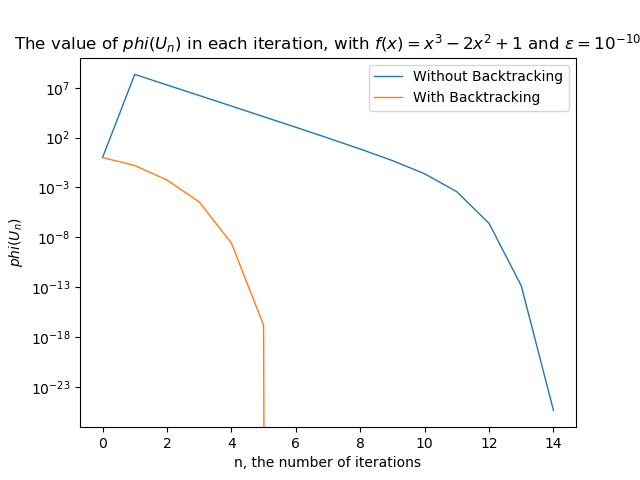
\includegraphics[width=0.5\textwidth]{backtracking_testing.png}
    \caption{Comparison of the value of $\Phi(U_n)$ with and without backtracking}
\end{figure}

\newpage
\section{Computation of the Lagrangian points}

\begin{flushright}
By Simon Bullot
\end{flushright}

In celestial mechanics, the Lagrangian points are points near two objects where a lighter object will remain at the same place relatively to the two other masses. The Newton-Raphson method is used to find these points.

\subsection{Forces implementation}

First, a function which takes two parameters will return another function representing centrifugal, elastic or gravitational force. For instance, a function g will return the centrifugal force function corresponding to the parameters $k$ and $X_0$.
\[g:k,X_{0} \mapsto f with f : X = (x,y) \mapsto (k(x-x_{0}),k(y-y_{0}))\]


Then another function would return Jacobian matrix for any of the forces needed.

\subsection{Newton-Raphson method application}

A third function will represent the sum of the forces by adding the desired gravitational and centrifugal forces. The same is done by another function for the matrix representing Jacobian forces sum matrix. Then the Newton-Raphson algorithm is used to find a point where forces are equal to zero. A point where sum forces are equal to zero will be an equilibrium point. In fact, due to Newton's first law, if an object does not have any velocity, and the forces acting on it are compensating themselves, then it will not move.

\subsection{Obtaining the Lagrangian points}

By running the Newton-Raphson algorithm with different $U_{0}$ points, different Lagrangian points can be found.
For instance, if those points are used :
\[U_0 = (0.5, 0), U_1 = (1.5, 0), U_2 = (-1.5, 0) \]
The algorithm will respectively find these points:
\[L_0 = ( 0.85927766, 0 ), L_1 =  (1.15775715, 0 ), L_2 = (-0.99754112, 0 ).\] 

\newpage
\section{Electrostatic equilibrium}
\begin{flushright}
By Imad Boudroua and  Mohammed Boudali
\end{flushright}

The purpose of this section is to show the equilibrium position of N charges placed in an electrostatic field. The movement studied is limited between -1 and 1 on the real axis.
\subsection{Algorithm to compute the Jacobian matrix}
The first step is to  compute the derivative of total  electrostatic energy function:
\begin{equation}
    E(x_1,..,x_N) = \sum_{i=1}^{N} ( \log(|x_i + 1| + \log|x_i - 1| + \frac{1}{2}\sum_{\substack{j=1 \\ j\neq i}}^{N} \log|x_i - x_j| )
\end{equation}
    After derivation, the expression found is:
\begin{equation}
\frac{\partial  E(x_1, ..,x_N)}{\partial x_i}
   = \frac{1}{x_i - 1}
      + \frac{1}{x_i + 1}
      + \sum_{\substack{j=1 \\ j\neq i}}^{N}\frac{1}{x_i - x_j}
      \end{equation}
Therefore, the elements of Jacobian matrix: $(\frac{\partial \nabla E_i}{\partial x_j})_{_{i,j}}$ can be simplified to: 

\vspace{5pt}

\[J_{i,j} = \begin{cases} -\frac{1}{(x_i - 1)^2} -\frac{1}{(x_i + 1)^2} - \sum_{\substack{j=1 \\ j\neq i}}^{N}\frac{1}{(x_i - x_j)^2} &\mbox{if } i\neq j \\
-\frac{1}{(x_i - x_j)^2} & \mbox{if }  i = j \end{cases}
\]


\subsection{Application of Newton-Raphson method}
    After using the Newton-Raphson method to solve the equation: $\nabla E(x_1, ..,x_n) = 0$,  the variation of energy gradient was plotted (Figure 2):
    
    
    \begin{figure}[!htb]
    \centering
    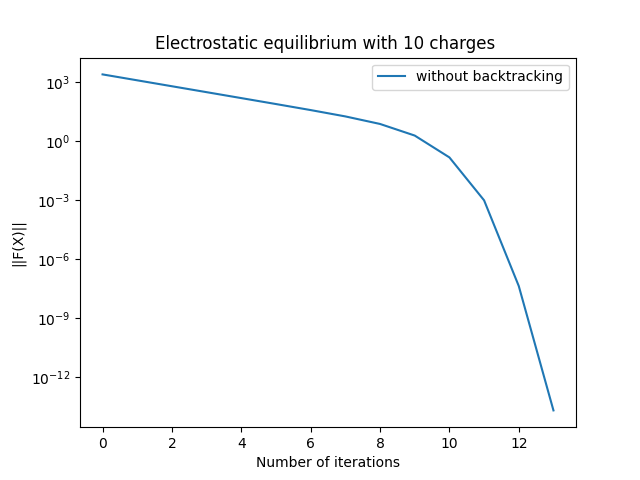
\includegraphics[width=0.7\textwidth]{equilibrium.png}
    \caption{Electrostatic equilibrium with 10 charges}
\end{figure}
\vspace{1cm}

\newpage
In Figure 2, the curve converges to 0. This result proves that the system studied reached an electrostatic equilibrium. This property is more noticeable in Figure 3:
\vspace{1cm}

    \begin{figure}[!h]
    \centering
    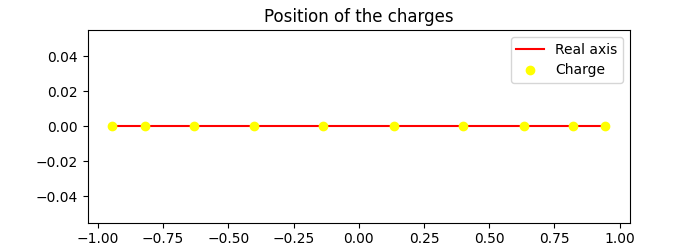
\includegraphics[width=0.7\textwidth]{position_real_axis.png}
    \caption{Position of the charges on the real axis}
\end{figure}


\subsection{Comparison with the Legendre polynomial derivative roots }
In this section, the functions \textbf{legder}, \textbf{leg2poly} and \textbf{poly1d} were used to draw the curve of Legendre polynomial. Equilibrium positions were plotted in the same figure in order to compare the results (Figure 4):

 
    \begin{figure}[!h]
    \centering
    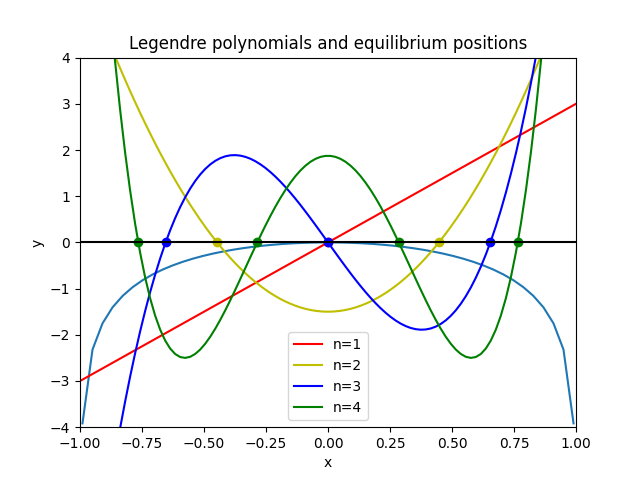
\includegraphics[width=0.8\textwidth]{legendre_comparaison.png}
    \caption{Legendre polynomials and equilibrium positions}
\end{figure}

This figure shows that Legendre polynomial derivative roots coincide with the equilibrium positions.
\subsection{The nature of the extremum}
The results show that electrostatic equilibrium positions reached a critical point. To determine its nature, the curve in Figure 5 was drawn.
    \begin{figure}[!h]
    \centering
    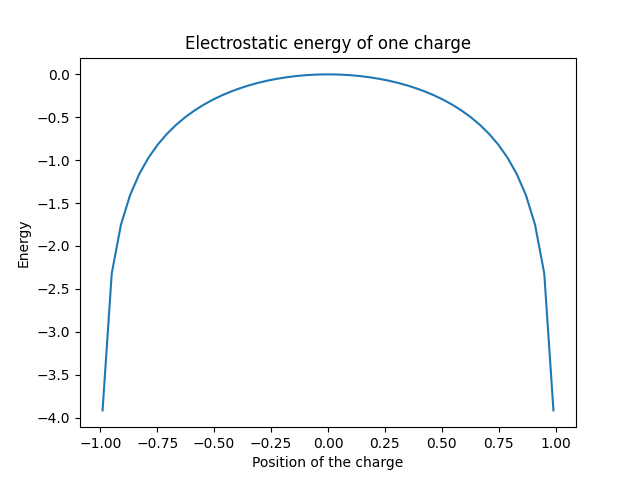
\includegraphics[width=0.7\textwidth]{energy_position.png}
    \caption{Energy variation of one charge on  [-1;1]}

\end{figure}
\newpage
   This curve is characterized by one global maximum reached in $x=0$.
   
\section{Conclusion}
\begin{flushright}
By Simon Bullot, Imad Boudroua and Lucas Guédon
\end{flushright}

The Newton-Raphson method can be a useful and powerful tool especially with the problems encountered in this project. In those cases, the Jacobian matrix of each function can be easily calculated. This enables the use of this method which works in any dimension. Moreover, the convergence of the algorithm studied is quadratic because roots are non stationary points and do not have multiplicity greater than one.

\end{document}
